\documentclass{article}
\usepackage[utf8]{inputenc}

\usepackage{mathtools}
\usepackage{amsthm}
\usepackage{graphicx}

\usepackage{listings}
\usepackage{xcolor}
\usepackage{cancel}
\usepackage{amssymb}

\usepackage[T1]{fontenc}

\title{FYS-MEK1110 Oblig 3}
\author{Samuel Bigirimana}

\begin{document}
    \maketitle
    \raggedright
    \section*{task a) the position \(s(t)\) given \(l_0 = 0.5m\)}
    By: \(t = 0 \), \(L_0 = 0.5m \) and \(h = 0.3\):
    \begin{equation*}
        \begin{split}
            0.5m &= \sqrt{(0.3m)^2+(x_0)^2} \\
               x_0 &= \sqrt{(0.5m)^2-(0.3m)^2} \\
                    &= \underline{\underline{0.4m}}
        \end{split}
    \end{equation*}

    \section*{task b) deciding the spring length given any position}
    The block will only move on the x-axis, this means that the spring can´t 
    be shorter than the hight difference between the block and the attachment point. 
    So the only movement the block makes is alongside the x-axises given a given time: \linebreak
    \begin{equation*}
        l = \sqrt{(0.3)^2+(x(t))^2}
    \end{equation*}

    \section*{task c) drawing the forces on the block:}
    \begin{center}
        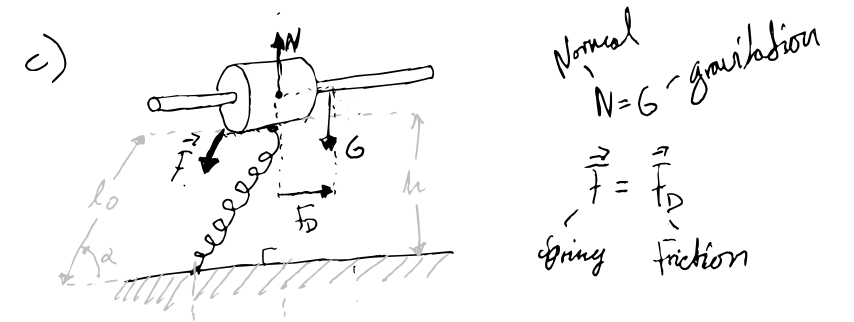
\includegraphics[scale=0.8]{../c.png}\linebreak
    \end{center}

    \section*{task d) proving the force in x-direction}
    As the springforce is given as \(F = -k(r-L_0)\dfrac{r}{r}\) and if we decomponise it in 
    x-direction, we get:
    \begin{equation*}
        \begin{split}
            F_x &= -k(r-L_0)\dfrac{x}{r} \\
                &= -k(\dfrac{rx}{x}-\dfrac{L_0x}{r}) \\
                &= -k(x-\dfrac{L_0x}{r}) \\
                &= -kx(1-\dfrac{L_0}{r}) \\
                \\
                r &= \sqrt{x^2 + y^2} \\
                \Rightarrow y &= h \\
                \\
                \Rightarrow F_x &= -kx(1-\dfrac{L_0}{\sqrt{x^2+h^2}})
        \end{split}
    \end{equation*}

    \section*{task e) plotting \(F_x\) given position in x-direction}
    › The program I made to build the plot:
    \lstinputlisting[language=Python]{../fx_plot.py}
    \pagebreak
    › The plot results for \(F_x\):
    \begin{center}
        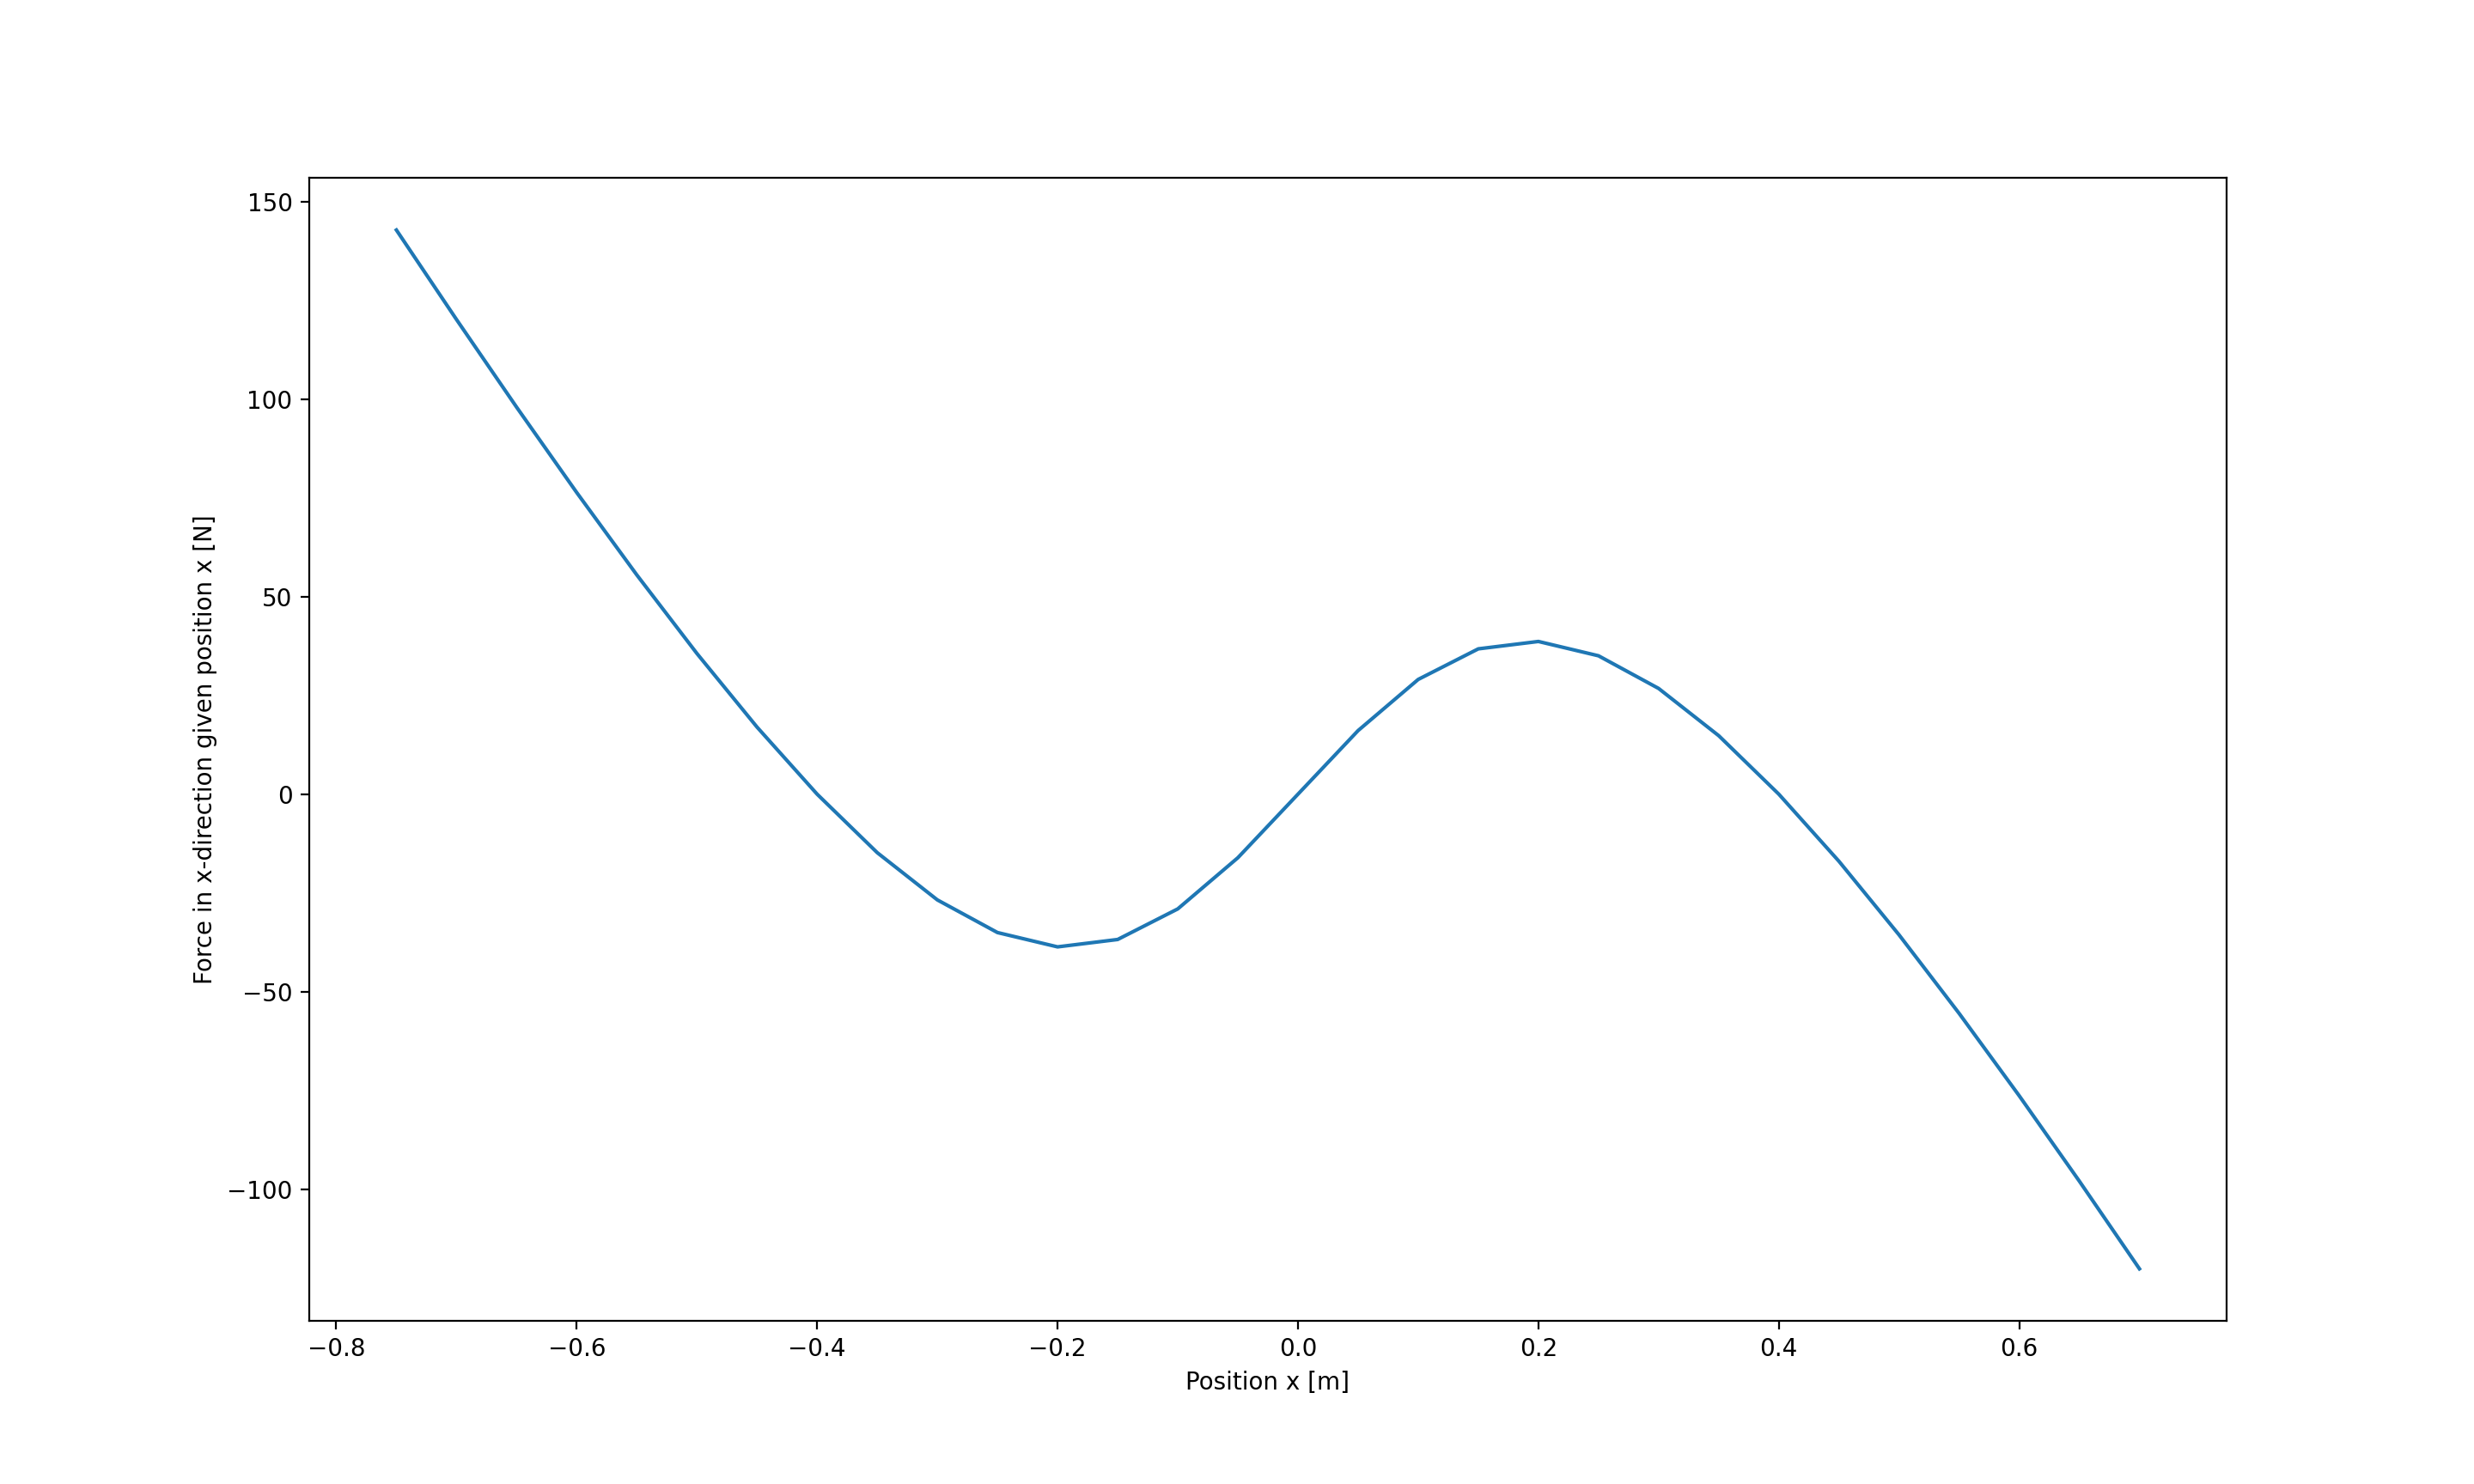
\includegraphics[scale=0.45]{../fx-plot.png}\linebreak
    \end{center}

    \section*{task f) solving the equations of motion numerically using the Euler-Cromer method given \(x1 = 0.6m \)}
    \lstinputlisting[language=Python]{../block.py}
    \pagebreak
    › The resulting plot:
    \begin{center}
        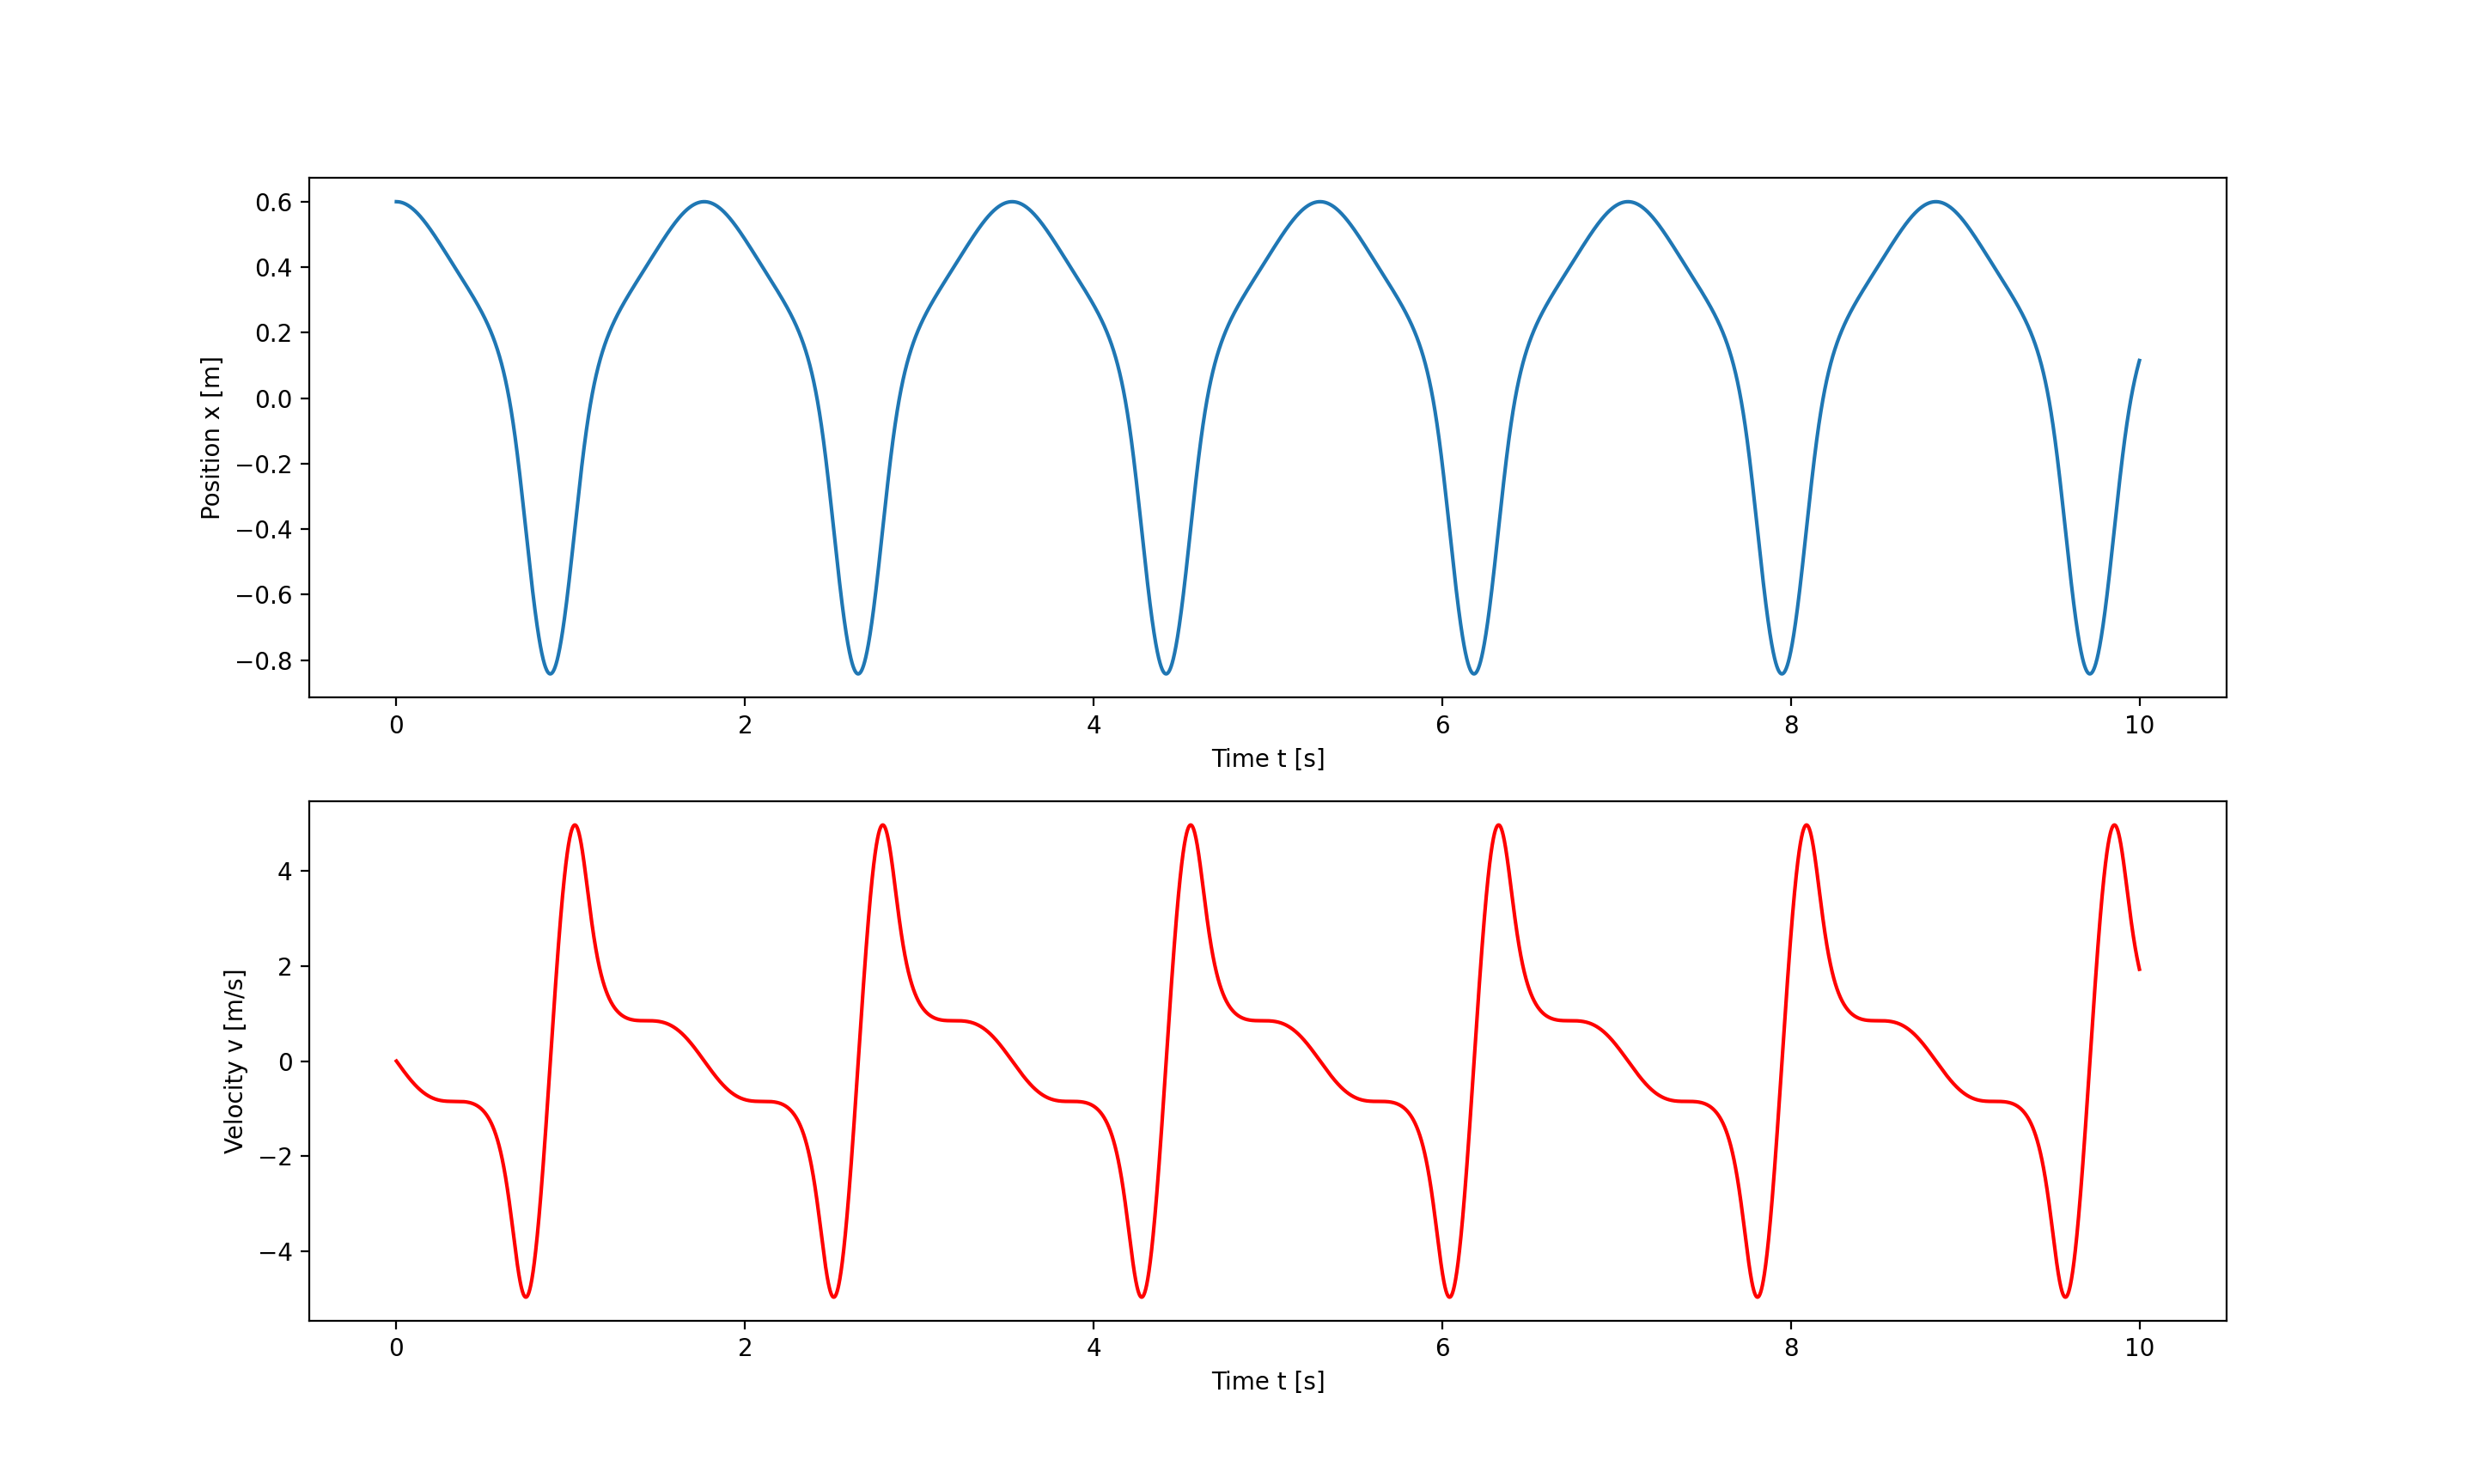
\includegraphics[scale=0.45]{../block.png}\linebreak
    \end{center}

    \section*{task g) solving the equations of motion numerically using the Euler-Cromer method given \(x1 = 0.65m \)}
    \lstinputlisting[language=Python]{../block2.py}
    \pagebreak
    › The resulting plot:
    \begin{center}
        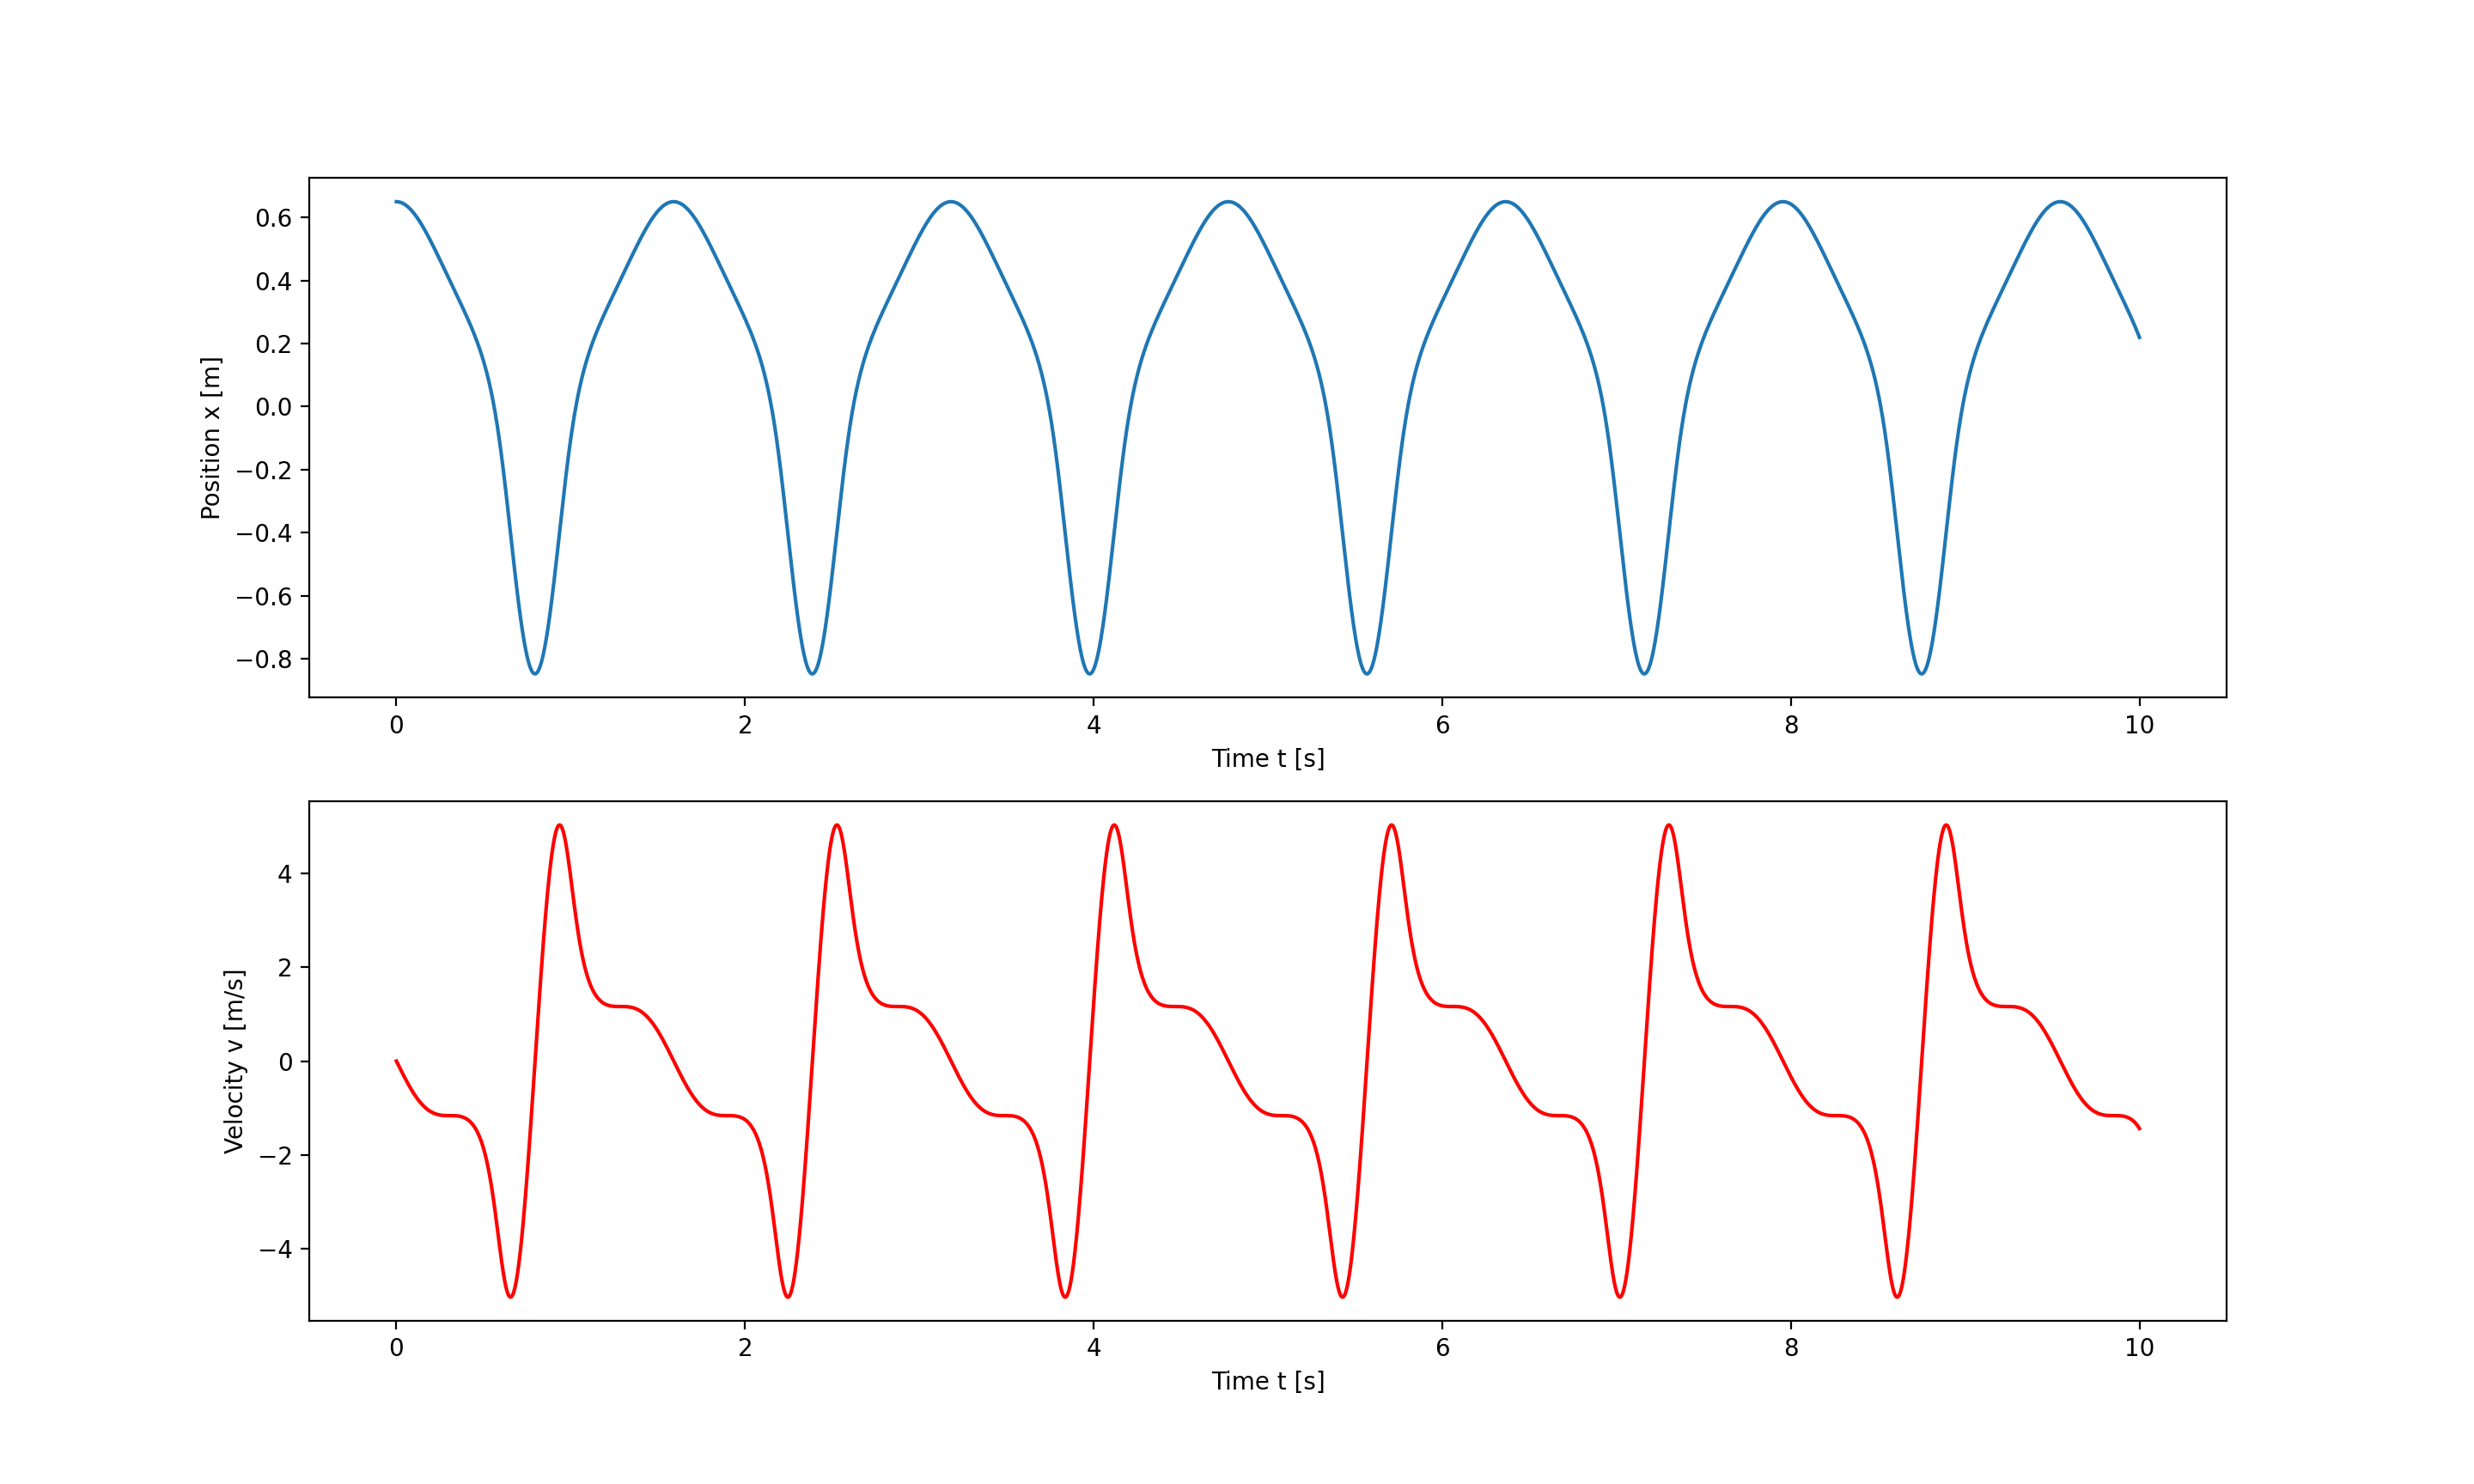
\includegraphics[scale=0.45]{../block2.png}\linebreak
    \end{center}

    \section*{task h) proving the force in y-direction }
    \begin{equation*}
        \begin{split}
            F_y &= -k(r-L_0)\dfrac{h}{r} \\
                &= -k(\dfrac{rh}{h}-\dfrac{L_0h}{r}) \\
                &= -k(h-\dfrac{L_0h}{r}) \\
                &= -kh(1-\dfrac{L_0}{r}) \\
                \\
                r &= \sqrt{x^2 + y^2} \\
                \Rightarrow y &= h \\
                \\
                \Rightarrow F_y &= -kh(1-\dfrac{L_0}{\sqrt{x^2+h^2}})
        \end{split}
    \end{equation*}

    \section*{task i) deciding the neutral force N: }
    Since the block is stand still by \(t = 0 \), N has to be the same size as the gravitational size (G): \linebreak
    \(N = G = mass * gravitational acceleration = 5kg * 9.81m/s^2 = \underline{\underline{49N}}\)

    \section*{task j) profing N(x): }
    If the sum of all forces on the block is equal to 0 (the block is standing still), we get:
    \begin{equation*}
        \begin{split}
            \sum{F} &= 0 \\
            N + (-G) + (-kh(1-(\dfrac{L_0}{\sqrt{x^2+h^2}}))) &= 0 \\
            \Rightarrow N(x) - m*g &= kh(1-(\dfrac{L_0}{\sqrt{x^2+h^2}})) \\
            N(x) &= kh(1-(\dfrac{L_0}{\sqrt{x^2+h^2}})) + m*g
        \end{split}
    \end{equation*}

    \section*{task k) drawing the forces on the block with friction:}
    \begin{center}
        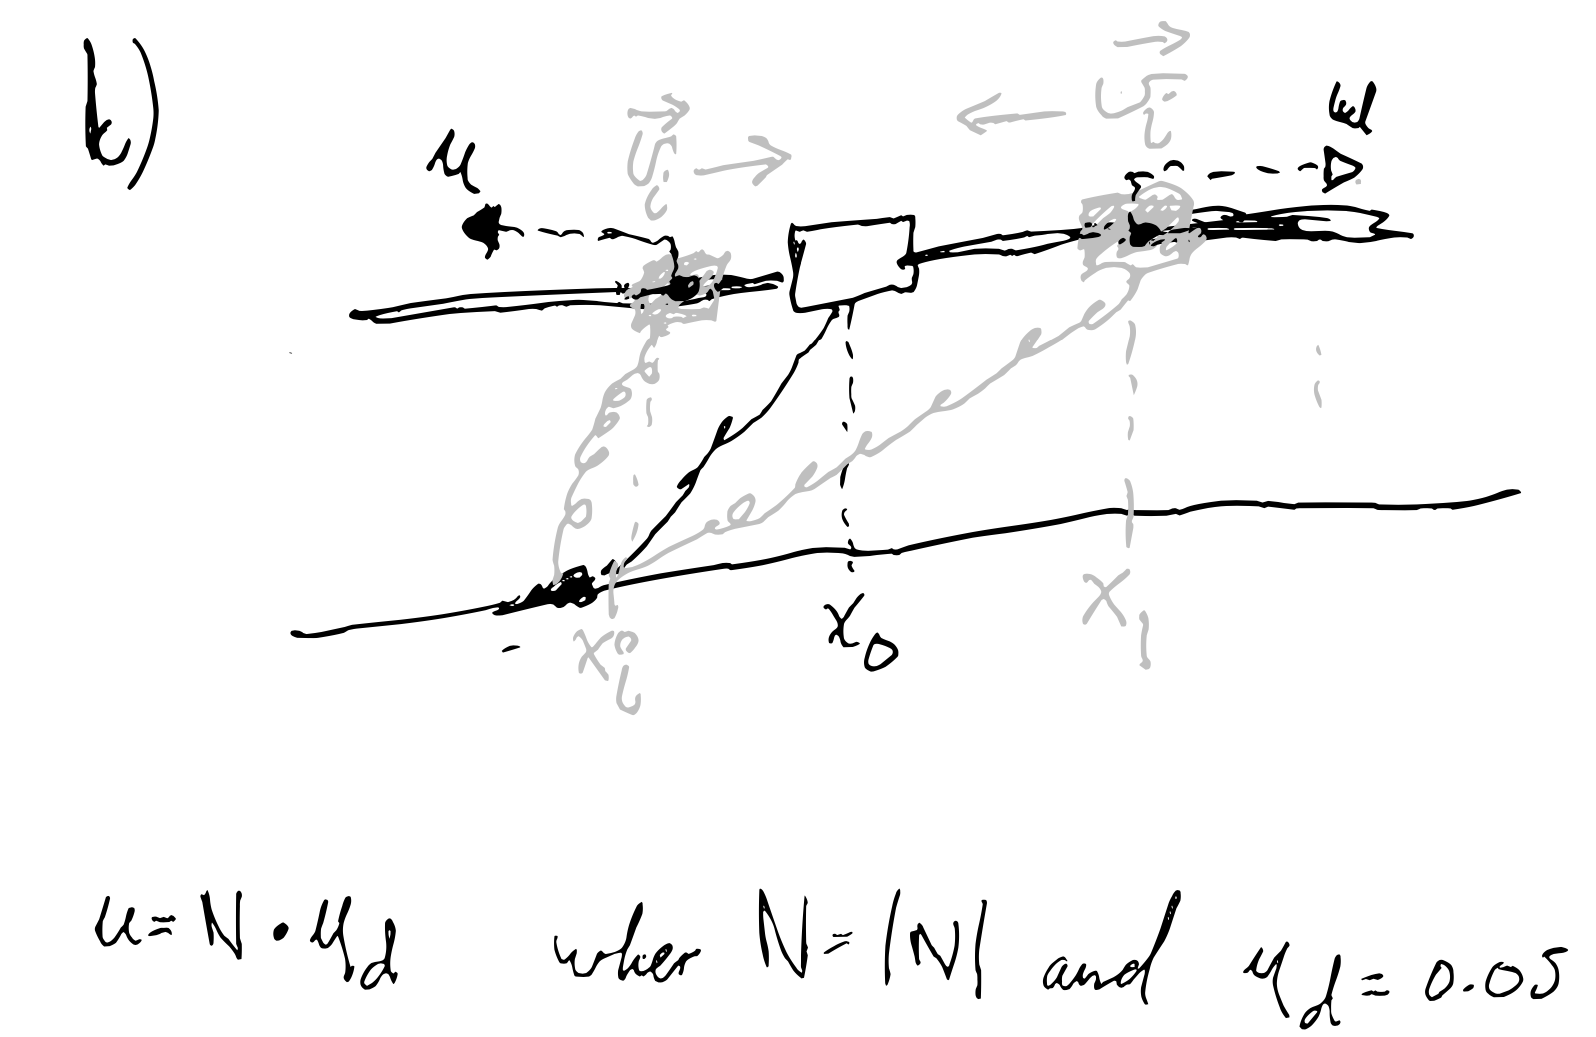
\includegraphics[scale=0.45]{../k.png}\linebreak
    \end{center}
    \pagebreak
    › The program for task k and i:
    \lstinputlisting[language=Python]{../block2.py}

    › The resulting plot:
    \begin{center}
        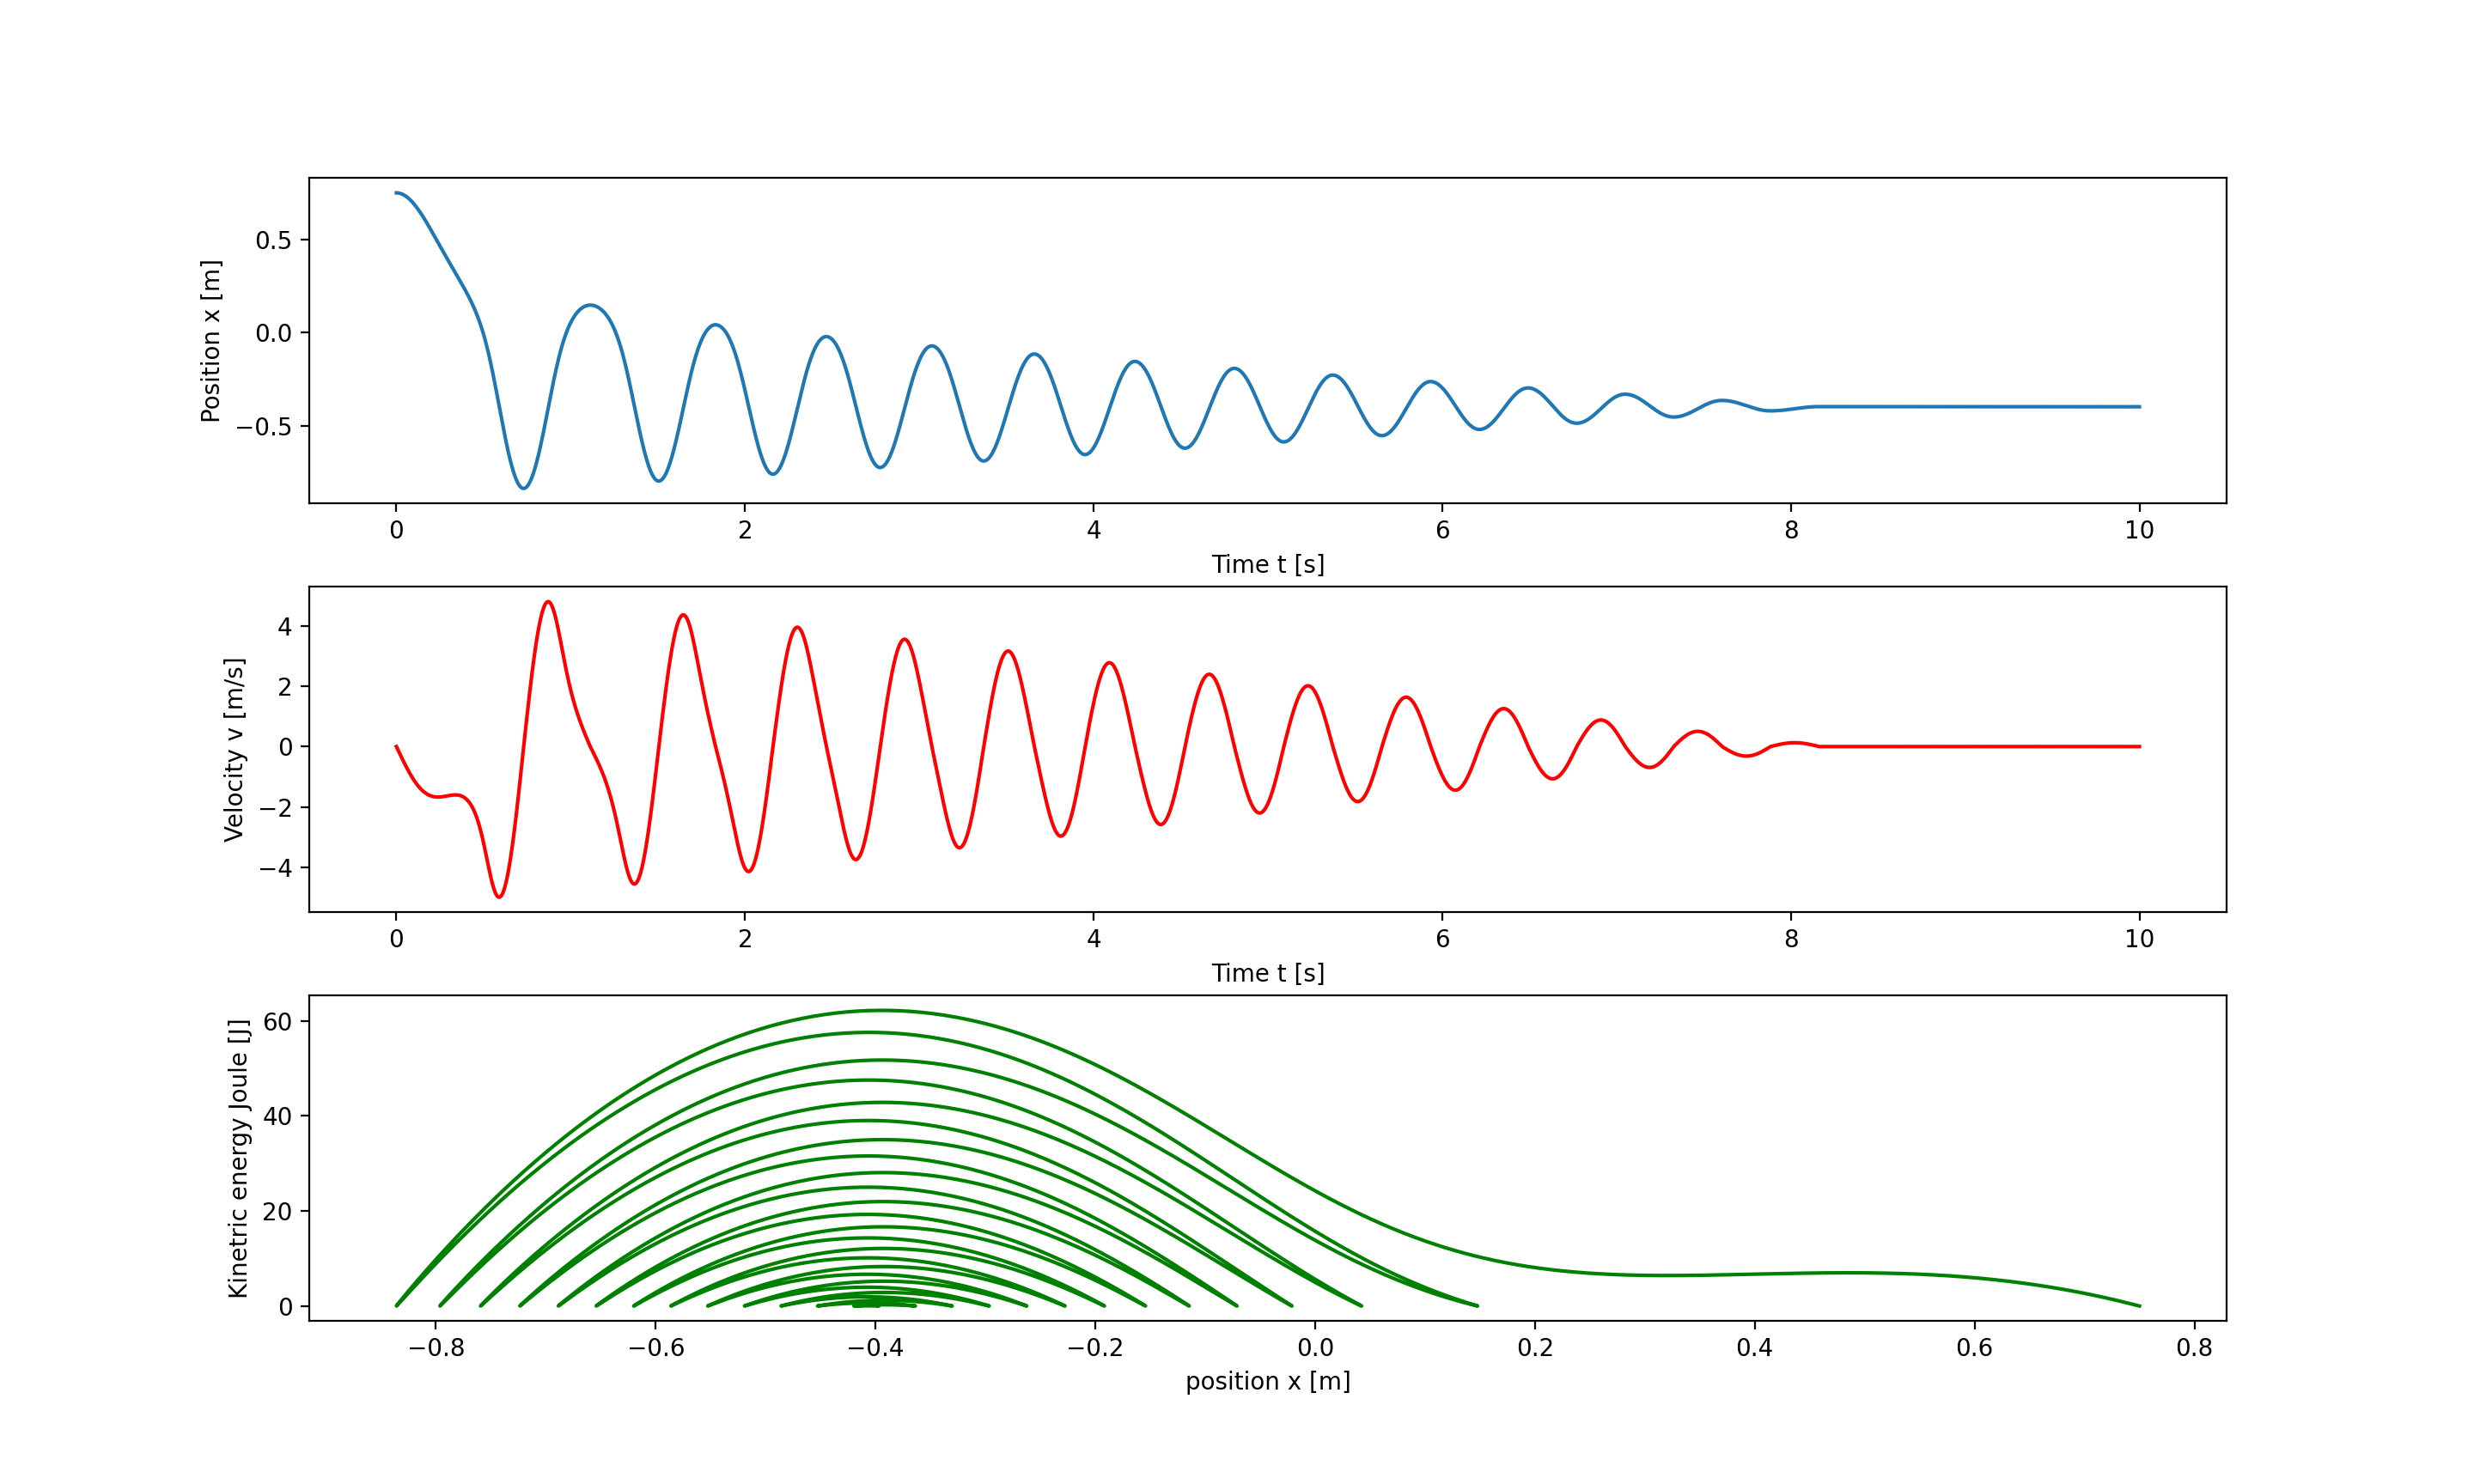
\includegraphics[scale=0.45]{../block3.png}\linebreak
    \end{center}

    › Task k; as we can see from the plot, the block´s movement is now getting braked by the friction.
    The force is not preserved and the movement stops. \linebreak
    › Task l: the last graph shows the kinetric energy given a position x. As we can see, the energy is at 
    its´highest when the block is right above the neutral position \(X_0\). This is becausen the movement has 
    its highest velocity by the point.

    \section*{task m) finding the equilibrium points}
    By looking at the plot for the kinetric energy, we can see that the equilibrium points for this equation 
    are 0.4m and -0.4m on the x-axis. \linebreak
    \begin{center}
        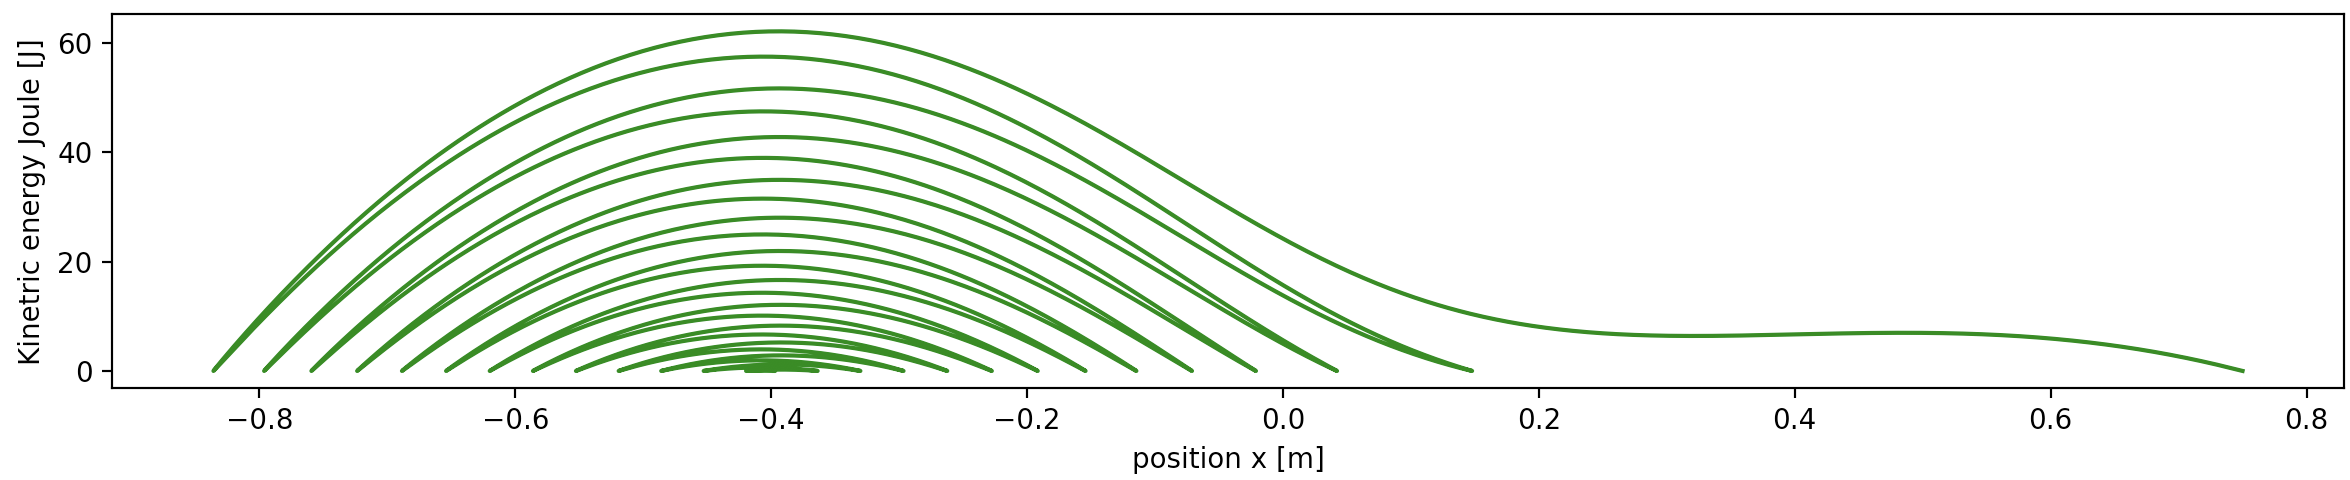
\includegraphics[scale=0.4]{../balance.png}
    \end{center}
\end{document}